The system is composed of three primary components, a cross-platform mobile application for viewing and sharing architectural models using AR, a database for storing augmented reality models and sessions and finally, a CRUD web application for managing and uploading models to the database. 

\section{Database}
For the purpose of this project, Firebase was used to store and sync data. The reason it was selected was for its NO-SQL, real-time data synchronization - a feature key to implementing shared AR. 

\subsection{Cloud Firestore}
Firestore is used to host and store the architectural models used in the application. The web client accesses firestore to create, read, update and delete these models. Models can be uploaded to the database using the uploadToStorage function provided by the Firebase plugin. 

\begin{minted}
[
baselinestretch=1.2,
fontsize=\footnotesize,
linenos
]
{java}
  // send file and name to data store
    let upload = this.dataProvider.uploadToStorage(text, file);

\end{minted}

\subsection{Realtime Database}
FIrebase’s real-time database is used to store data pertinent to the mobile application. The application’s database has two primary data stores - one for storing  AR sessions and another for storing the URLs that point to the architectural models located in the cloud firestore databse.

\begin{figure}[ht!]
\caption{Database Schema}
\centering
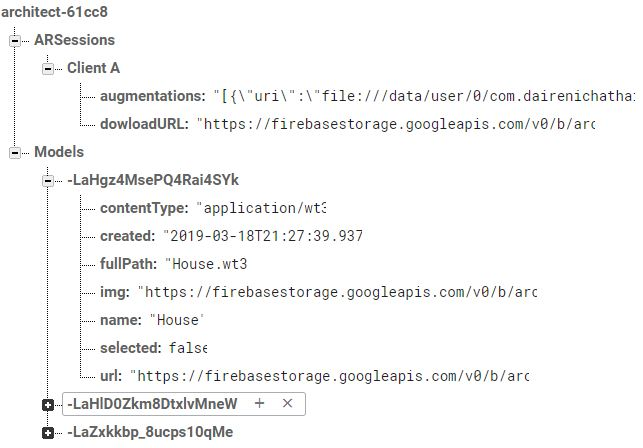
\includegraphics[scale=0.55]{images/firebase_databse.JPG}
\end{figure}


\section{Web Application}
The web application functions as a tool for managing the architectural models used in the mobile application. In a real-world use case, the architect or product owner would have access to the web client, and from here, could organise the models they wish to share with customers. 

The web app leverages Firebase’s Cloud Firestore database to host the models, which take the form of .wt3 files. The user interface facilitates full CRUD behaviour, allowing the user to create, read, update and delete any files located in the application’s database.

The web client is a single page application built using the Ionic framework. The root page of the application presents all the .wt3 files currently stored in the database.

\begin{figure}[ht!]
\caption{Web Application}
\centering
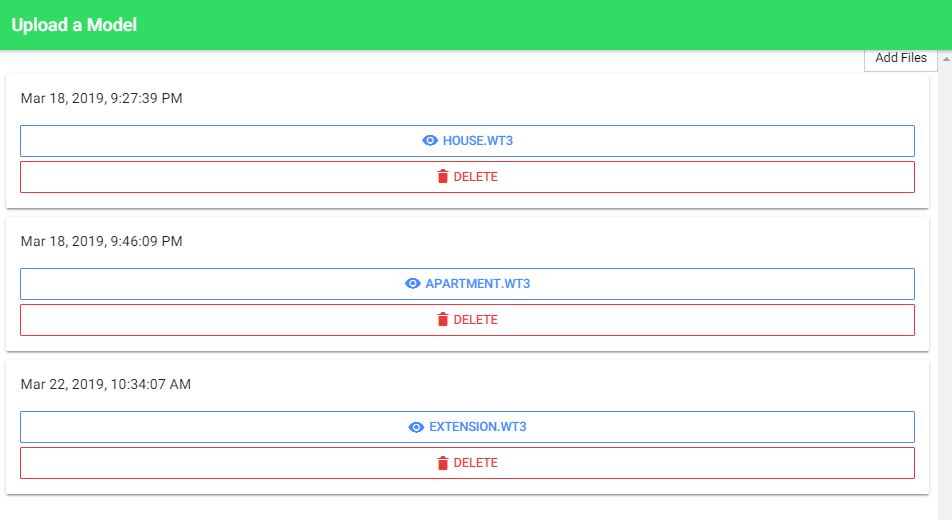
\includegraphics[width=1\textwidth]{images/web_client.JPG}
\end{figure}


\begin{itemize}
    \item The Add Files button utilises the Apache Cordova file picker plugin to allow the user to select a local file to upload.
    
    \item Clicking a the files triggers an instant download to the user’s device. This feature can be used to preview a model on the user’s local device. 

    \item The delete button removes the file from the database. A popover confirms the successful deletion of a file. \\ \\
\end{itemize}



\section{Mobile Application}

The objective of the mobile application is to provide the user with a tool to preview architectural models through the use of augmented reality. 

An example use case would be an architect and customers discussing and designing plans for a new construction. As illustrated by \cite{lorensen1987marching}, people often find it difficult to visualize 3D models in physical space without sufficient visual aids. This mobile application would serve to aid architects in expressing their designs to customers. The architect creates a session that clients can join. In this session, an architectural model can be shared between parties, enabling multiple users to interact with virtual content in the same real-world location that can be seen on different devices, in the same position and orientation relative to the environment. This way, the proposed model can be viewed and interacted with, promoting a collaboration and a common understanding between users. 


\subsection{Home Page}

This is the root page of the application. From here the user may proceed with one of the following options, creating a new AR Session or loading a previously saved session. These options are presented in the form of two buttons.

\begin{figure}[ht!]
\caption{Home Page}
\centering
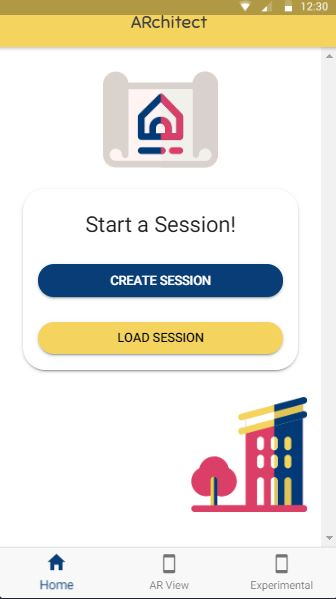
\includegraphics[scale=0.65]{images/home_page.JPG}
\end{figure}


\begin{itemize}
    \item Selecting the \say{Create Session} button triggers navigation to the \say{Create Session Page}.
    
    \item Selecting the \say{Load Session} button triggers the Load Session Popover. 

\end{itemize}



\subsubsection{Load Session Popover}
The Load Session popover features a single input field to allow the user to enter a session name. 


\begin{figure}[ht!]
\caption{Load Session Popover}
\centering
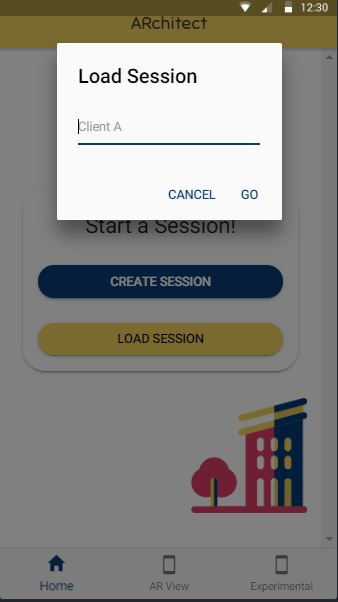
\includegraphics[scale=0.55]{images/load_session_popover.JPG}
\end{figure}

\begin{itemize}
    \item The \say{Go} button then checks the database for any AR sessions with a matching name. If it fails to find a match, a popup is used to inform the user.
    
    \item If a match is found, the AR session is loaded from the database and written device file system. 
    
    \item
    The model required in the AR session is written to a .wt3 file on the file system.

    \item
    Once all the required resources are loaded from the database, the user is navigated to the \say{AR} View page. \\ \\
    
    
\end{itemize}



\subsection{Create AR Session Page}
On this page, the user is presented with an input form to provide details for the creation of a new AR Session.

\begin{figure}[!ht]
\caption{Create AR Session Page}
\centering
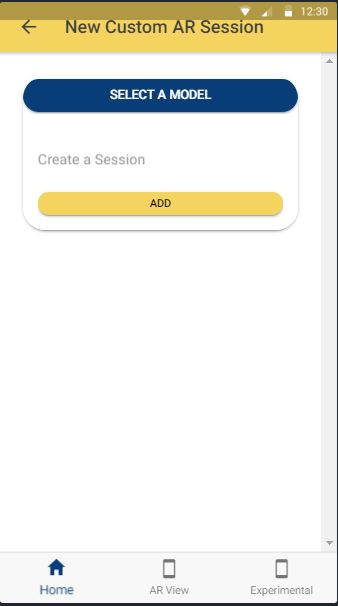
\includegraphics[scale=0.55]{images/create_session_page.JPG}
\end{figure}

\begin{itemize}

    \item The \say{Select a model} button opens a modal displaying architectural models that can be selected to use in the shared AR session. Model information is dynamically loaded from the database. The model information contains the model title, thumbnail image and a URL to the storage location of the .wtc file in the database. 

    \item The input field allows the user to specify a name for the session. This name becomes the session key which can be shared with other users wishing to engage in the same AR session.
    
    \item The \say{Add button} triggers the creation of the AR session. An entry is made in the database using the session name as an object key. The selected model is then downloaded using the model URL and written locally to the device storage. 

    
\end{itemize}


\subsection{AR View}
This page is used to present the AR content. The ARchitect world is initialized so that augmented content can be rendered.

\begin{figure}[!ht]
\caption{ARView Page}
\centering
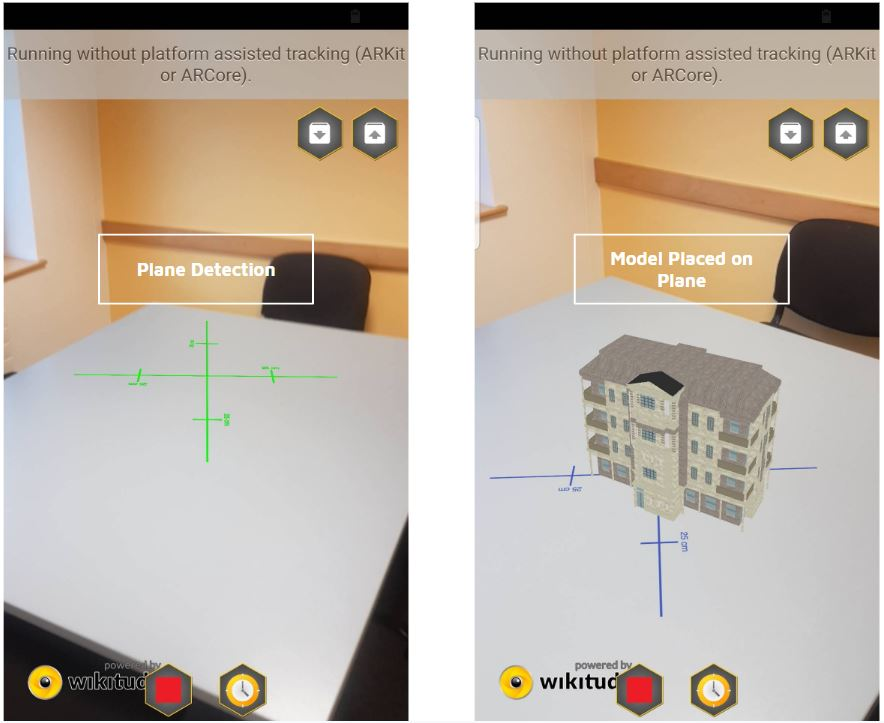
\includegraphics[scale=0.55]{images/arview_page.JPG}
\end{figure}

\begin{itemize}
    \item To place a model within the scene the user must first detect a plane. The cross-hair drawable is used to aid the user in detecting a plane. 

    \item The slider can be used to adjust the cross-hair size so that the plane can be scaled up or down depending on the users preference. 
    
    \item Once a valid plane is identified, the cross-hair changes from red to green. The user must then tap to anchor the plane. The user can then place a model on the plane by tapping the area they wish to plant it.
    
    \item The user can interact with the model via a drag gesture to move it or pinching to scale. The model can also be rotated with a select and drag gesture.
    
    \item Any alterations made to the model are updated to the database in real-time. Any other users connected to the same session will see the updates made to model. 


\end{itemize}


\subsection{Experimental Page}
 This page serves to highlight Wikitude's Scene Detection Functionality. 
 \begin{itemize}
     \item The camera can be used to scan the environment for a predefined Object Trackable(scene). 
     \item Once the scene is recognised, an architectural model is placed within the scene, using the model's specified scale, rotation and orientation.
 \end{itemize}



\subsection{Scene Detection}
Scene detection is implemented using Wikitude's Object Recognition and Scene Detection functionality. An object tracker was created using Wikitude Studio. This was achieved by uploading a selection of images representing the area to be recognised. Wikitude Studio was then used to place a model within the defined area. Following this, the tool generates the .wto (Wikitude Object Trackable file). This file was then added to mobile application. The  \say{Experimental Page} within the app illustrates Scene Recognition in action. 

\subsection{Shared AR}
Shared AR is implemented using Wikitude's Persistent Tracking functionality. To create a shared AR session, a unique session key must be provided by the user. Following this, an entry is created in the \say{ARSessions} object in the database. Once an instance of an InstantTrackable is in the tracking state and a model is associated with it, the database begins listening for updates to the AR scene. 
\\  
The user can interact with the AR scene via altering the model’s scale, rotation and orientation. Any changes in the AR session trigger an update in the database. These changes are propagated to all other users interacting with the same AR session. In a similar way, if another user creates a change in the scene, the current user’s AR scene will be updated to reflect it. Firebase’s real-time database is used to facilitate the live syncing of ar scenes. 
\\  \\
When loading the AR Scene, its JSON representation is pulled from the database and written to a file locally. The writing of this file is achieved through the use of the Apache Cordova File plugin.


\begin{minted}
[
baselinestretch=1.2,
fontsize=\footnotesize,
linenos
]
{javascript}
// get access to file system
    window.resolveLocalFileSystemURL(cordova.file.externalDataDirectory, function(fs) {
        // get the file, if it doesn’t exist, create it
        fs.getFile("SavedAugmentations.json",
          { create: true, exclusive: false },
          function(fileEntry) {
            // instantiate the writer
            fileEntry.createWriter(function(writer) {
            // write the augmentation json object loaded from DB
              writer.write(augmentations);
            }
          }
              }

\end{minted}

An instance of the FileWriter Object is created. The augmentations loaded from the database are then written to the SavedAugmentations.json file. Due to security restrictions on Android Devices, the device’s external data directory is the only directory used for reading and writing content within the application. 
